% section Evaluation
\label{sec:eval}
\vspace*{-5pt}

We now present the experimental evaluation of our caching-based keep-alive and provisioning techniques by using function workload traces and serverless benchmarks.
Our goal is to investigate the effectiveness of the these techniques under different workload and system conditions. 



\begin{figure*}
  \centering
    \vspace*{\myfigspace}
\subfloat[ Representative functions.     \label{fig:rep-trace-exec}]
{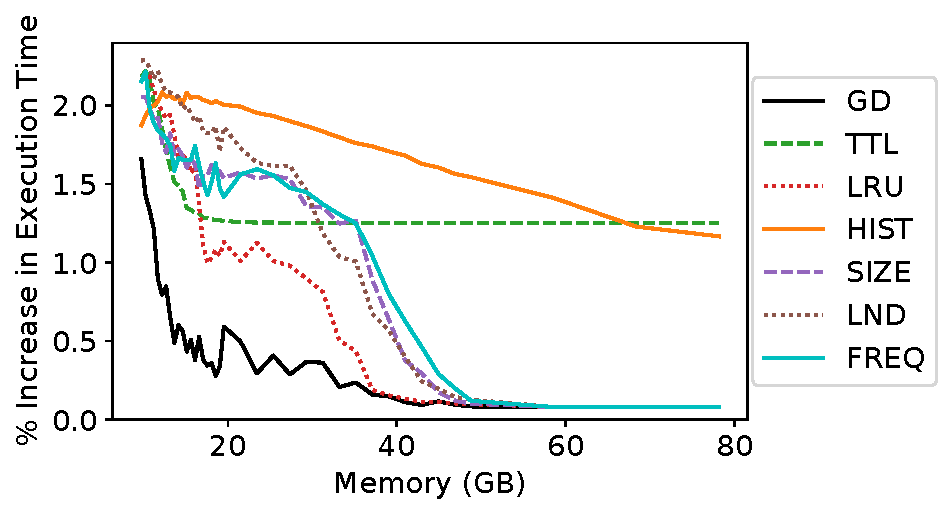
\includegraphics[width=0.35\textwidth]{../graphs/rep-funcs-392/exec_inc_mem-392-legend.pdf}}
  \hfill 
    \subfloat[Rare functions.     \label{fig:rare-trace-exec}]
{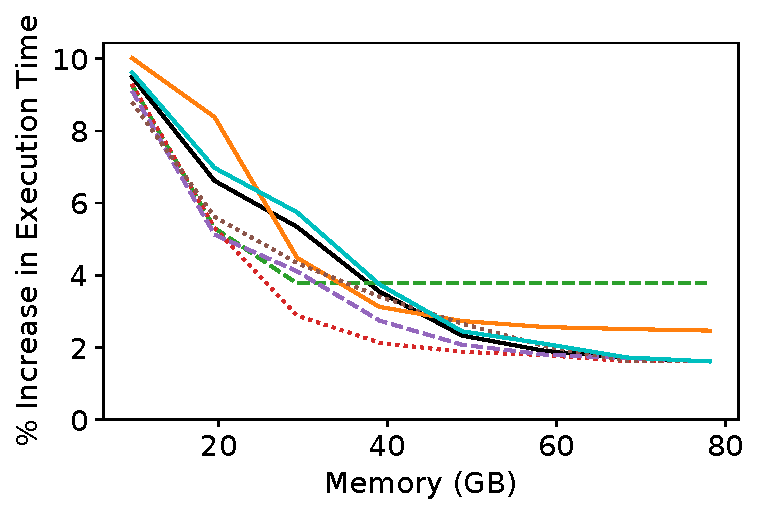
\includegraphics[width=0.27\textwidth]{../graphs/rare-funcs-1000/exec_inc_mem-1000.pdf}}
\hfill 
  \subfloat[Random sampling.      \label{fig:random-trace-exec}] {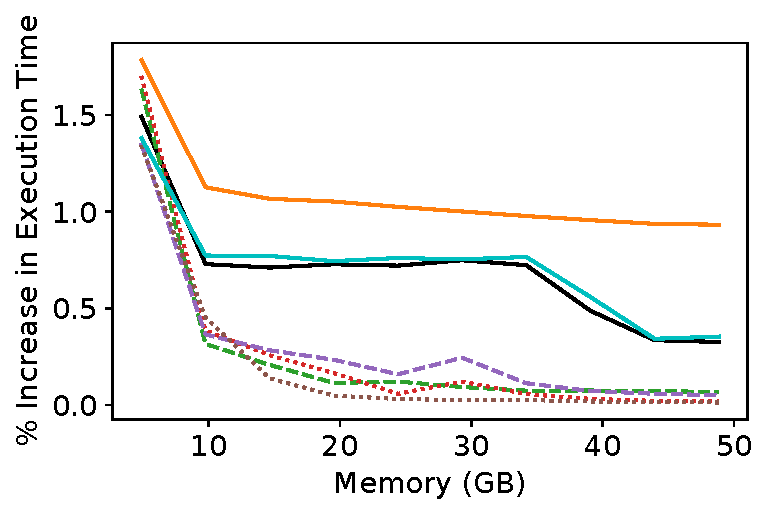
\includegraphics[width=0.27\textwidth]{../graphs/random-funcs-200/exec_inc_mem-200.pdf}}
  \vspace*{\myfigspace}
\caption{Increase in execution time due to cold starts for different workloads derived from the Azure function trace.}
\label{fig:exec-overheads-all}
  \vspace*{\myfigspace}
\end{figure*}


\begin{figure*}[t]
  \centering
%  \vspace*{\myfigspace}
  \begin{minipage}[c]{0.7\linewidth}
  \subfloat[Representative functions.\label{fig:rep-trace-cold}] {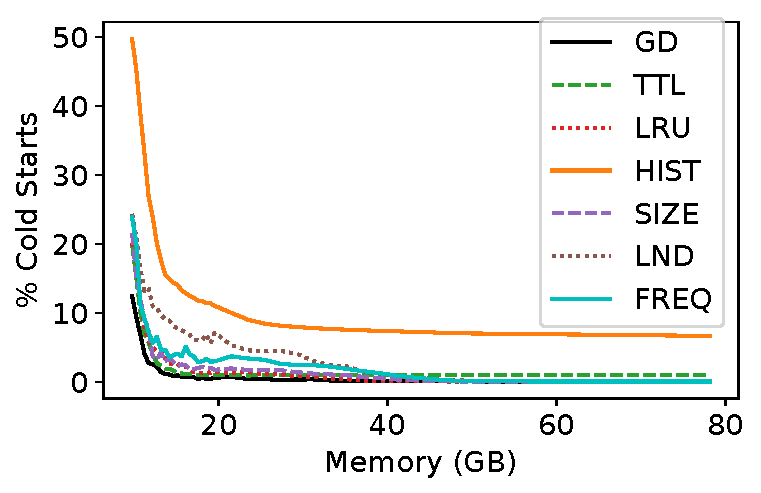
\includegraphics[width=0.3\textwidth]{../graphs/rep-funcs-392/cold_drop_mem-392-legend.pdf}}
  \hfill
    \subfloat[Rare functions. \label{fig:rare-trace-cold}] {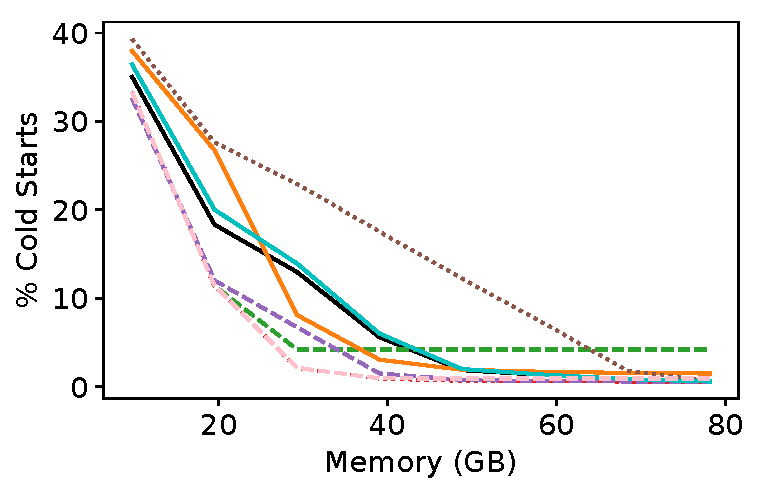
\includegraphics[width=0.3\textwidth]{../graphs/rare-funcs-1000/cold_drop_mem-1000.pdf}}
  \hfill
  \subfloat[Random sampling. \label{fig:random-trace-cold}]
  {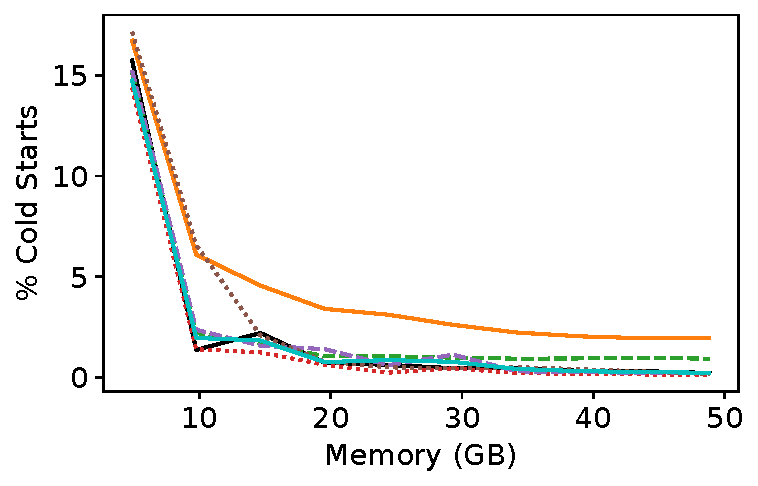
\includegraphics[width=0.3\textwidth]{../graphs/random-funcs-200/cold_drop_mem-200.pdf}}
    \vspace*{\myfigspace}
    \caption[cold starts]{Fraction of cold starts is lower with caching-based keep-alive. } % for different samples of the Azure function trace.}
      \vspace*{\myfigspace}
      \label{fig:cold starts-all}
    \end{minipage}
    \hfill
    \begin{minipage}[c]{0.29\linewidth}
 %      \begin{figure}
      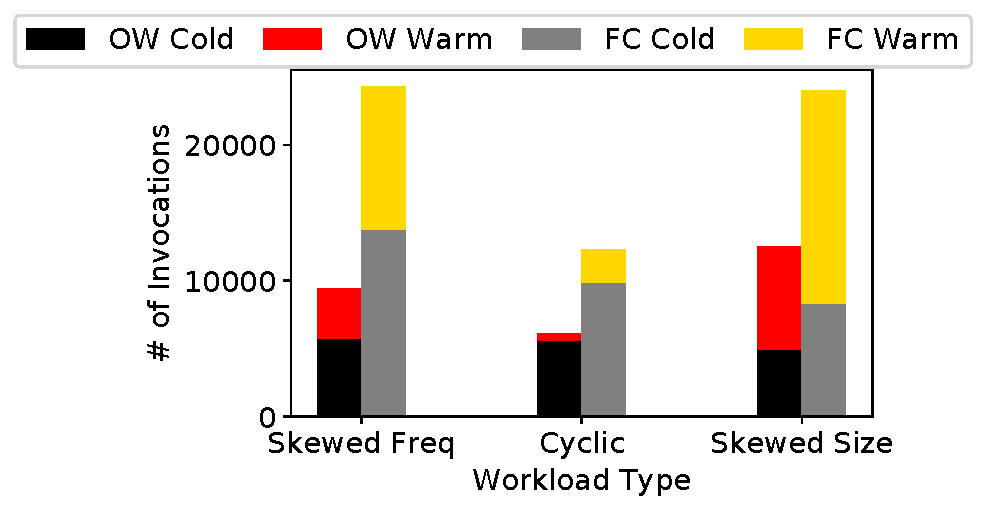
\includegraphics[width=1\textwidth]{../graphs/litmus_tests/litmus_2_stacked.pdf}
      \caption{FaasCache runs 50 to 100\% more cold and warm functions, for skewed workload traces.}
              \label{fig:litmus_2}
 %     \end{figure}
    \end{minipage}
\end{figure*}


%%%%%%%%%%%%%%%%%%%%%%%%%%%%%%%%%%%%%%%%%%%%%%%%%%%%%%%%%%%%
\noindent \textbf{Setup, Workloads, and Metrics.}
%
For evaluating different keep-alive performance with different workload types, we use different trace samples from the Azure Function trace~\cite{shahrad_serverless_2020}, which contains execution times, memory sizes, and invocation-timestamps for more than 50,000 unique functions. 
Since our goal is to examine performance at a \emph{server} level, we use smaller samples of this trace for realistic server sizes, and replay them in our discrete-event keep-alive simulator. 
This also allows us to examine the behavior with different \emph{types} of workloads, which is important because our keep-alive policies are designed to be general and workload-agnostic.
We use the following three trace samples (more details in the Appendix): \\
\noindent \textbf{RARE:} A random sample of 1000 of the rarest, most infrequently invoked functions. This is similar to the evaluation workload used in~\cite{shahrad_serverless_2020}.  \\
\noindent \textbf{REPRESENTATIVE:} A sample of 400 functions, sampled from each quartile of the dataset based on frequency---yielding a more representative sample with higher function diversity. \\
\noindent \textbf{RANDOM:} A random sample of 200 functions. 


\begin{comment}
Our simulator evaluation uses real-world FaaS usage data from the recently released Azure Function trace~\cite{shahrad_serverless_2020}. 
%
The entire trace consists of tens of thousands of functions with billions of invocations, making it intractable to simulate the entire dataset.
%
Trace sampling methodology is important to capture the characteristics of the overall trace, and the scenarios where FaasCache is most effective.
%
Over half of all functions have an interval arrival time (IAT) over 30 minutes, guaranteeing them to always have cold starts when using a simple TTL eviction policy. 
%
A tiny 1\% of functions account for nearly 90\% of all invocations, with an IAT of under a minute. 

% Therefore, smaller samples 
Given these extreme disparities, smaller samples must match behaviors of the larger dataset to show their effectiveness.
%
The full Azure trace can be suitably handled by a cluster of servers, in which case the system behavior is influenced by load-balancing and sharding policies, which our work is orthogonal to.

% Explain the rationale here. 
We generate three day-long traces using the Azure Functions dataset to showcase the effectiveness of FaasCache.

\prat{Insert reuse distance vs. time heatmaps for all these traces in the appendix along with table describing: number of fns, total invocations, avg. inter arrival time, etc.}

\end{comment}

We are interested in two metrics: the cold start ratio; and the average increase in the execution time due to cold starts. 
The latter captures the heterogeneity in function initialization overheads and invocation frequencies. 
For estimating the initialization overhead of each function using the workload trace, we subtract each functions' average runtime from its maximum runtime. 

%%%%%%%%%%%%%%%%%%%%%%%%%%%%%%%%%%%%%%%%%%%%%%%%%%%%%%%%%%%%
\subsection{Trace-driven Keep-alive Evaluation}
\vspace*{\subsecspace}
% In this subsection, we use the Azure function traces to evalaute different keep-alive policies in our discrete-event simulator.

% Primary Comparison? Competitors? 
We compare all caching-based variants against the default keep-alive policy in OpenWhisk (10 minute TTL). 
We also compare against the histogram based keep-alive policy in~\cite{shahrad_serverless_2020}, which is the state of the art technique. 
We have reproduced this policy (HIST) from the details in the paper, and have implemented it in a ``best-effort'' manner without any knowledge of the optimizations in the actual implementation. 
This is effectively a ``TTL+Prefetching'' policy: it uses a histogram of inter-arrival times to predict future function invocations. 
We also evaluate different Greedy-Dual variants: GD is our GDSF policy described in Section~\ref{subsec:gdsf}.
The others are the caching-based variants described in Section~\ref{subsec:variants}: LND is Landlord, and FREQ is LFU. 
%
The increase in execution time for different traces and for different cache sizes is shown in Figure~\ref{fig:exec-overheads-all}.
% How is this measured?
The increase in execution time is the cold start overheads averaged across all invocations of each function, and captures the user-visible response-time. 
%

For the representative trace (Figure~\ref{fig:rep-trace-exec}), Greedy-Dual reduces the cold start overhead by more than $3\times$ compared to TTL for a wide range of cache sizes (15--80 GB). 
Interestingly, it is able to achieve a low overhead of only 0.5\% at a much smaller cache size of 15GB, compared to other variants, which need 50 GB to achieve similar results---a reduction of cache size by more than $3\times$. 
%
For rare functions (Figure~\ref{fig:rare-trace-exec}), caching-based approaches such as LRU  reduce the cold start overhead by $2\times$ compared to TTL for cache sizes of 40--50 GB. 
This shows that for rare functions, recency is a more pertinent characteristic, and the complex four-way tradeoff used in Greedy-Dual is not necessarily ideal in all workload scenarios. 
For this workload, the HIST policy outperforms TTL, as reported in~\cite{shahrad_serverless_2020}. 
However, it results in 50\% higher cold start overhead compared to caching-based approaches.
Furthermore, because HIST uses only inter-arrival times, it is unable to perform well with heterogeneous representative workloads  (Figure~\ref{fig:rep-trace-exec}). 


Finally, the randomly sampled trace has a large number of infrequent functions because of the low probability of selecting the heavy-hitting functions.
In Figure~\ref{fig:random-trace-exec}, the recency component again dominates, and we see LRU outperforming other variants. 
The equivalence of LRU and TTL-based caching for rare objects is well established~\cite{basu2017adaptive,jiang2018convergence}, which explains their similar behavior seen in Figure~\ref{fig:random-trace-exec}. 
%closeness of TTL and LRU performance for rare functions in our result. 

\noindent \emph{\textbf{Result:} For representative, diverse workloads, our GD policy can improve the performance and shrink cache sizes by up to $3\times$. For more homogeneous workloads, LRU can outperform current TTL-based approaches by $2\times$.}

We see a similar relation and behavior in the miss-ratio curves shown in Figure~\ref{fig:cold starts-all}.
Due to function heterogeneity, the cold start overheads are not strictly correlated with cache miss ratios, and thus the differences between policies is different compared to the previously described actual cold start overheads. 
% \prat{Write after colors are fixed.}
We note that the average inter-arrival time for all three workloads is less than 36ms. As the IAT grows, the effectiveness of work-conserving caching-based approaches increases compared to TTL, as we shall see next. 

%%%%%%%%%%%%%%%%%%%%%%%%%%%%%%%%%%%%%%%%%%%%%%%%%%%%%%%%%%%%
\subsection{OpenWhisk Evaluation}
\vspace*{\subsecspace}

We now evaluate the performance of our FaasCache keep-alive implementation, and compare it to the vanilla OpenWhisk system which uses a 10 minute TTL. 
By leveraging Greedy-Dual caching, FaasCache is able to reduce cold starts. 
This also reduces the number of \emph{dropped} requests. % Why?
OpenWhisk buffers and eventually drops requests if it cannot fulfill them.
Because FaasCache more effectively selects evictions, its higher hit rate results in functions finishing faster, allowing more functions to be executed in the same time frame.  
%
To examine the effect of Greedy-Dual keep-alive on cold start and dropped requests, we use a small workload trace comprising of four different functions: Disk-bench, ML inference, Web-serving, and Floating-point from Table~\ref{tab:workloads}.

In Figure~\ref{fig:litmus_2}, we use different kinds of \emph{skewed} workloads: with a single function having a different frequency, a cyclic access pattern, and a skewed workload with 2 sizes. 
We see that FaasCache's keep-alive can increase the number of warm invocations by between 50 to 100\% compared to OpenWhisk's TTL.
The difference in the total number of requests served (warm+cold) is because OpenWhisk drops a significant number of requests due to its high cold start overhead and resultant system load. 
%Interestingly, OpenWhisk drops a significant number of requests, which is the cause of the different total served requests. 
%

% The impact on the different function performances can be seen in Figure~\ref{fig:faasbench}.
% For this figure, to generate the workload, the first three functions have an inter-arrival time of 1500 ms, and the fourth (floating-point) has a lower IAT of 400 ms. 

%a disk-based one, web-page serving, floating-point trigonomotry operations in numpy, and a convolutional neural network inference (TensorFlow with which model?). % A detailed description of these workloads is required.

% Explain what is the iat distribution and (other details? ).


% 32 GB wted_increase vanilla 11.964% cache 11.528%
% 48 GB wted_increase vanilla 6.184% cache 0.624%


\begin{figure}[t]
  \centering
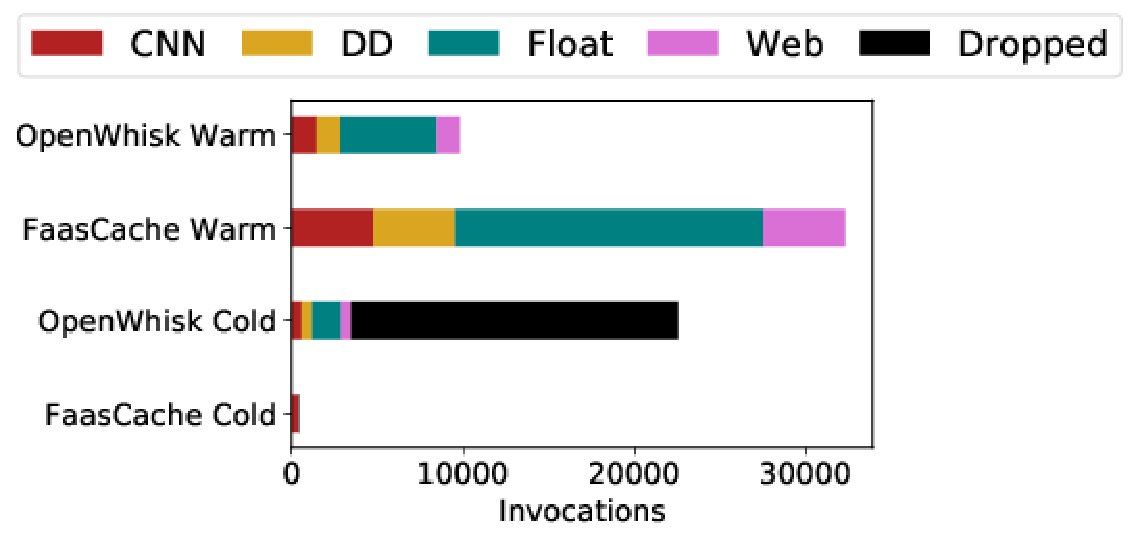
\includegraphics[width=0.4\textwidth]{../graphs/litmus_tests/faasbench_48_cold_hot-legend.pdf}
\caption{FaasCache increases warm-starts by more than $2\times$, which also reduces system load and dropped functions.}
\label{fig:faasbench}
\end{figure}


\begin{comment}
\begin{figure}[t]
  \centering
\subfloat[48 GB   \label{fig:faasbench-stacked-48}]
{ 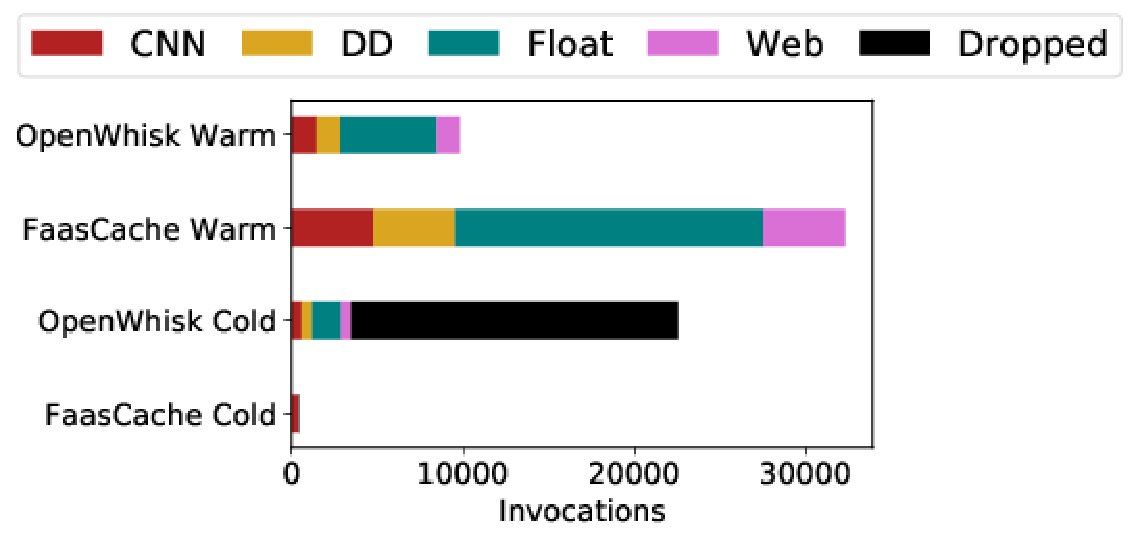
\includegraphics[width=0.3\textwidth]{../graphs/litmus_tests/faasbench_48_cold_hot-legend.pdf}}
\hfill 
  \subfloat[32 GB   \label{fig:faasbench-stacked-32}]
{  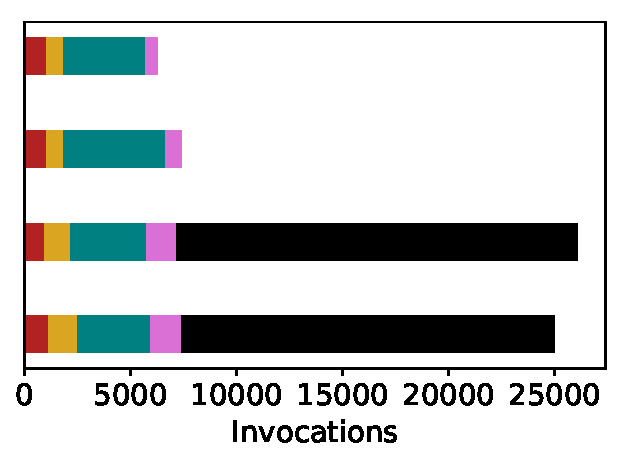
\includegraphics[width=0.17\textwidth]{../graphs/litmus_tests/faasbench_32_cold_hot.pdf}}
\caption{Impact of keep-alive on different function types.}
\label{fig:faasbench}
\end{figure}
\end{comment}

% Figure~\ref{fig:faasbench-stacked-32} shows the number of cold and dropped requests for the different functions, with a medium cache size of 32 GB.
% This setup is intended to evaluate our system in resource constrained environments.
% We see that dropped requests dominate, and FaasCache's more effective keep-alive serves 45\% of requests, while OpenWhisk only serving ~40\%.
% At the same time, warm starts improve 17\% using FaasCache.


Next, we use the skewed frequency workload and use functions from Table~\ref{tab:workloads} to evaluate the impact on real applications. 
%The impact on the different function performances can be seen in Figure~\ref{fig:faasbench}.
To generate the workload, the CNN, DD, and Web-serving functions have an inter-arrival time of 1500 ms, and the Floating-point function has a lower IAT of 400 ms. 
%
Figure~\ref{fig:faasbench} shows the breakdown of different function invocations for this workload on a 48 GB server.
Interestingly, OpenWhisk drops a significant number (50\%) of requests due to the its high cold start overheads.
FaasCache increases the warm requests by more than $2\times$. 
Interestingly, the \emph{distribution} of warm starts is also different. 
FaasCache's Greedy-Dual policy prioritizes functions with higher initialization times, but penalizes those with large memory footprints.
Because the floating-point function has a high initialization overhead (Table~\ref{tab:workloads}), it sees a $3\times$ increase in hit-ratio compared to OpenWhisk.
\emph{In practical terms, the improvement in keep-alive results in a $6\times$ reduction in the application latency.
}
%The ML inference function has an 8\% lower warm hit rate than the other functions, as it gets de-prioritized because of it's high memory needs.


%When the cache size is increased to 48 GB (Figure~\ref{fig:faasbench-stacked-48}), FaasCache doesn't drop a single request, while OpenWhisk still can't serve 50\% of them.
%For the same workload, Figure~\ref{fig:faasbench-stacked-32} shows the distribution of cold and warm starts for a larger cache size of 32 GB.
%The number of warm starts increases by nearly 20\% compared to OpenWhisk.
% FaasCache's Greedy-Dual policy prioritizes functions with higher initialization times, the CNN function sees a 53\% higher warm starts, wheres Z function only sees X\% increase compared to OpenWhisk. 
% The floating point function has a very high initialization overhead (1.7 of the total 2 seconds), and thus sees its warm-start rate increase the most, by 40\%. 

\begin{comment}
At a smaller cache size of 32 GB shown in Figure~\ref{fig:faasbench-stacked-32}, the number of dropped requests dominate.
This setup is intended to evaluate our system in resource constrained environments.
FaasCache's more effective keep-alive serves 45\% of requests, while OpenWhisk drops nearly 60\%.
Warm-starts increase by 17\% with FaasCache. 
\end{comment}

\noindent \emph{\textbf{Result:} FaasCache can increase the number of warm-starts by $2\times$ to $3\times$ depending on the function initialization overheads and workload skew. This results in lower system load, which increases the number of requests FaasCache can serve by $2\times$.}

%\prat{CPU Graph not required, but just the average numbers will do.}

%%%%%%%%%%%%%%%%%%%%%%%%%%%%%%%%%%%%%%%%%%%%%%%%%%%%%%%%%%%%
\subsection{Effectiveness of Provisioning Policies}
\vspace*{\subsecspace}
All our previous results have been with a statically allocated server, and 
we now illustrate the effectiveness of our dynamic vertical scaling policy described in Section~\ref{subsec:dynamic}.
The goal is to dynamically adjust the cache size based on the workload. 
Our  policy seeks to keep the miss speed (cold starts per second) close to a pre-specified target. 
This is shown in Figure~\ref{fig:dynamic}---the target is 0.0015 misses per second. 
In this experiment, the cache resizing is done only when the miss speed error exceeds 30\%, and we can see that the cache size increases with the miss speed, and decreases with it. 
Without the dynamic scaling, a conservative provisioning policy would result in a constant, 10,000 MB size. 
In contrast, the average cache size with our proportional controller is less than 7,000 MB.
This 30\% reduction means that FaaS providers can reduce their provisioned resources without compromising on performance.
The freed-up resources can be used to accommodate additional cloud workloads (such as co-located VMs and containers). 
Our dynamic scaling is extremely conservative: increasing its agressiveness by reducing the error tolerance below 30\% will reduce  average server size,
%but cause a larger number of small memory-size  changes, which we wish to avoid.
but we seek to avoid the resultant small changes to memory-size to minimize fragmentation. 
%avoid why?? 

\begin{figure}[t]
    \vspace*{\myfigspace}
  \centering 
  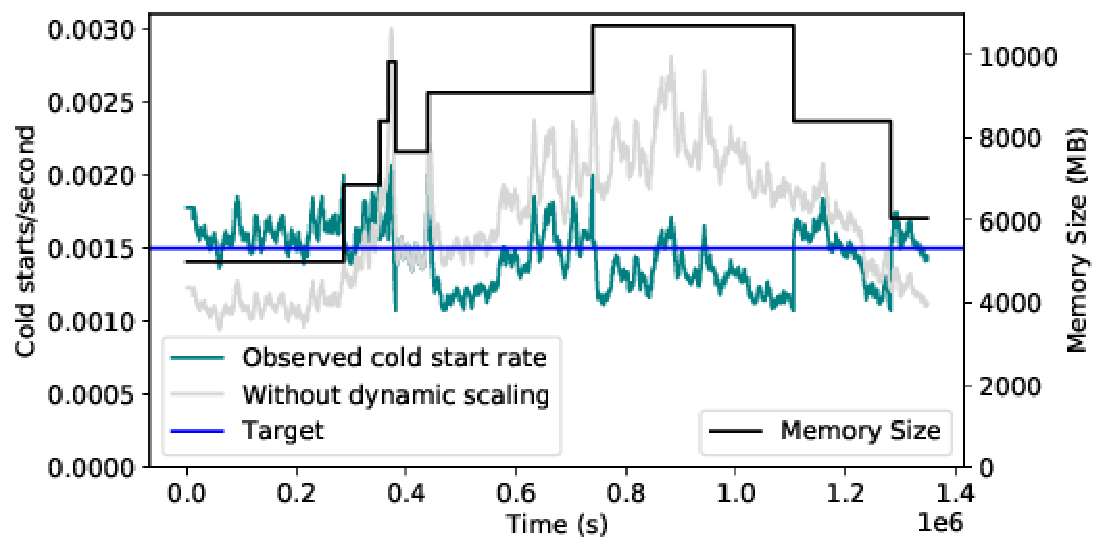
\includegraphics[width=0.4\textwidth]{../graphs/dyn-scale-392-b.pdf}
    \vspace*{\myfigspace}
  \caption{With dynamic cache size adjustment, the cold starts per second are kept close to the target (horizontal line), which reduces the average server size by 30\%. }
  \label{fig:dynamic}
  \vspace*{\myfigspace}
\end{figure}


%%% Local Variables:
%%% mode: latex
%%% TeX-master: "paper"
%%% End:
